% =============================================================
%  SABD 2025/26 - Project 1 Report
%  Author: Daniel Garoz
%  Institution: Universita degli Studi di Roma "Tor Vergata"
%  Format: IEEE Conference Proceedings (IEEEtran)
% =============================================================
\documentclass[conference]{IEEEtran}
\IEEEoverridecommandlockouts

\usepackage{cite}
\usepackage{amsmath,amssymb,amsfonts}
\usepackage{graphicx}
\usepackage{textcomp}
\usepackage{xcolor}
\usepackage{booktabs}
\usepackage{url}
\usepackage[hidelinks]{hyperref}
\usepackage{tikz}
\usetikzlibrary{positioning,arrows.meta,shapes.geometric,fit}
\usepackage{listings}

\lstset{
    basicstyle=\ttfamily\scriptsize,
    breaklines=true,
    columns=fullflexible,
    keywordstyle=\color{blue!70!black}\bfseries,
    commentstyle=\color{green!50!black}\itshape,
    stringstyle=\color{red!70!black},
    showstringspaces=false,
    frame=single,
    rulecolor=\color{gray!50},
    framesep=4pt,
    aboveskip=4pt,
    belowskip=4pt,
}

\def\BibTeX{{\rm B\kern-.05em{\sc i\kern-.025em b}\kern-.08em
    T\kern-.1667em\lower.7ex\hbox{E}\kern-.125emX}}

\begin{document}

\title{Distributed Analysis of US Airline Delays\\
using Apache Spark and HDFS}

\author{
\IEEEauthorblockN{Daniel Garoz}
\IEEEauthorblockA{
    M.Sc. Computer Engineering --- Erasmus Exchange\\
    Universit\`a degli Studi di Roma ``Tor Vergata''\\
    Rome, Italy
}
}

\maketitle

% -------------------------------------------------------------
\begin{abstract}
This report describes the design, implementation and experimental
evaluation of a Big Data processing pipeline that analyses on-time
performance data published by the US Bureau of Transportation
Statistics (BTS). The pipeline combines Apache Spark for distributed
processing and the Hadoop Distributed File System (HDFS) for
distributed storage, both deployed through Docker Compose so that
the entire stack can be reproduced from a single YAML file.
Two analytical queries are implemented with the Spark DataFrame API
and benchmarked in two configurations: a local PySpark environment
running directly on the host, and a fully containerized HDFS+Spark
cluster. Across five measured iterations the steady-state mean
execution time is $5.89$\,s (Q1) and $3.94$\,s (Q2) on the local
setup, against $19.09$\,s (Q1) and $17.27$\,s (Q2) on the cluster;
the $3.2$--$4.4\times$ gap is dominated by network shuffles,
HDFS metadata access and container startup. Beyond the numerical
results, the report makes a point of documenting \emph{why} every
non-trivial implementation choice was made --- explicit schema
declaration, selective caching, output coalescing, treatment of
NULL delay-cause columns --- so that the trade-offs behind each
decision remain traceable.
\end{abstract}

\begin{IEEEkeywords}
Big Data, Apache Spark, HDFS, Docker, Performance Evaluation,
Distributed Computing, Airline Delays.
\end{IEEEkeywords}

% -------------------------------------------------------------
\section{Introduction}

The growing availability of public, large-scale transportation
datasets makes it possible to study the operational behaviour of
the air transport sector with the same techniques employed in
industrial Big Data analytics. The US Bureau of Transportation
Statistics (BTS) in particular publishes a monthly on-time
performance dataset that contains every flight operated by
reporting carriers, including delay information broken down by
attributed cause~\cite{bts}.

This dataset is large enough --- on the order of two million
records for the four-month window January--April 2025 --- to
justify the use of a distributed processing framework rather than a
single-node pandas pipeline. Doing so in a controlled and
reproducible setup is the central objective of Project~1 of the
course \emph{Sistemi e Architetture per Big Data} (SABD),
A.A. 2025/26.

\paragraph{Goal}
The work pursues two complementary objectives: (i)~answering the
two pre-defined analytical queries (Q1 and Q2) over the BTS data,
and (ii)~doing so through a pipeline that respects the
architectural constraints stated in the project specification ---
specifically, reading the input from HDFS and writing the output
back to HDFS even when the team is a single student.

\paragraph{Contributions}
The report contributes (i)~a fully containerized HDFS+Spark stack
described in Section~\ref{sec:architecture}, (ii)~two Spark
DataFrame implementations of Q1 and Q2 (Section~\ref{sec:queries})
together with an explicit justification of every design decision,
and (iii)~a measured comparison between local PySpark execution
and the dockerized cluster (Section~\ref{sec:eval}).

\paragraph{Organization}
Section~\ref{sec:dataset} describes the dataset and a notable
constraint on its availability. Section~\ref{sec:architecture}
details the system architecture and the rationale behind the chosen
container stack. Section~\ref{sec:queries} discusses the two query
implementations. Section~\ref{sec:eval} presents the experimental
results. Section~\ref{sec:discussion} collects the observations
that I found most relevant while building the pipeline.
Section~\ref{sec:conclusion} concludes.

% -------------------------------------------------------------
\section{Dataset}\label{sec:dataset}

The pre-processed dataset distributed by the course is meant to
cover US domestic flights from January~1, 2025 to April~30, 2025
(approximately $2.2$~M events). The archive made available
through the course materials at the time of this work, however,
contains the first three months only --- January, February and
March 2025 --- which still amount to \textbf{1{,}554{,}583
flights} once the header rows are removed
(Table~\ref{tab:dataset-sizes}). All experimental results
presented in the rest of the report therefore refer to this
three-month subset. This is an acknowledged constraint that
does not affect the validity of the methodology: the queries
operate on whatever interval is loaded, so the same pipeline can
be re-run unchanged when the April archive becomes available.

\begin{table}[h]
\centering
\caption{Dataset breakdown after header removal.}
\label{tab:dataset-sizes}
\begin{tabular}{lrr}
\toprule
\textbf{Month} & \textbf{Records} & \textbf{Size (MB)}\\
\midrule
202501 (January)  & 539{,}747 & 61.5\\
202502 (February) & 504{,}884 & 58.0\\
202503 (March)    & 509{,}952 & 58.4\\
\midrule
\textbf{Total}    & \textbf{1{,}554{,}583} & \textbf{177.9}\\
\bottomrule
\end{tabular}
\end{table}

Each record contains 27 columns. To keep the computation cheap,
the loader projects only the 14 columns that are actually required
by Q1 and Q2: \texttt{YEAR}, \texttt{MONTH},
\texttt{DAY\_OF\_MONTH}, \texttt{OP\_UNIQUE\_CARRIER},
\texttt{CRS\_DEP\_TIME}, \texttt{DEP\_DELAY},
\texttt{ARR\_DELAY}, \texttt{CANCELLED}, \texttt{DIVERTED},
\texttt{CARRIER\_DELAY}, \texttt{WEATHER\_DELAY},
\texttt{NAS\_DELAY}, \texttt{SECURITY\_DELAY} and
\texttt{LATE\_AIRCRAFT\_DELAY}. Performing this projection at
load time (\emph{column pruning}) materially reduces I/O and
memory pressure, especially when the data has to travel over the
network from HDFS.

\paragraph{Treatment of NULL values}
The five delay-cause columns are frequently NULL. The BTS
convention is to populate them only when
\texttt{ARR\_DELAY}~$\geq 15$~minutes; in all other cases the
field is left empty. In this work the NULLs are coerced to zero
through \texttt{F.coalesce(col, F.lit(0.0))}. The interpretation
is straightforward: ``this cause did not contribute to the
delay''. The alternative of dropping rows with NULLs would
silently restrict the average to delayed flights only and bias
the mean upwards by roughly an order of magnitude, which is why
I rejected it.

% -------------------------------------------------------------
\section{System Architecture}\label{sec:architecture}

The deployment relies on Docker Compose to orchestrate four
containers running on a private Docker bridge network, sketched
in Fig.~\ref{fig:architecture}.

\begin{figure}[h]
\centering
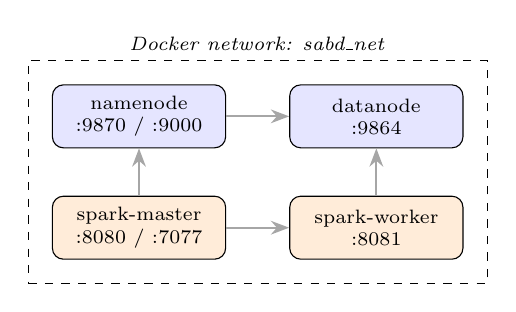
\begin{tikzpicture}[
    node distance=6mm and 8mm,
    box/.style={
        rectangle, draw, rounded corners, minimum height=8mm,
        minimum width=22mm, align=center, font=\scriptsize,
        fill=blue!10
    },
    sparkbox/.style={box, fill=orange!15},
    arrow/.style={-{Stealth}, thick, gray!70}
]
\node[box]      (nn) {namenode\\\scriptsize :9870 / :9000};
\node[box, right=of nn] (dn) {datanode\\\scriptsize :9864};
\node[sparkbox, below=of nn] (sm) {spark-master\\\scriptsize :8080 / :7077};
\node[sparkbox, right=of sm] (sw) {spark-worker\\\scriptsize :8081};

\draw[arrow] (nn) -- (dn);
\draw[arrow] (sm) -- (sw);
\draw[arrow] (sm) -- (nn);
\draw[arrow] (sw) -- (dn);

\node[draw, dashed, fit=(nn) (dn) (sm) (sw),
      inner sep=3mm, label=above:{\scriptsize \emph{Docker network: sabd\_net}}] {};
\end{tikzpicture}
\caption{Containerized deployment. HDFS (namenode + datanode)
provides storage; Spark (master + worker) provides compute. The
project source tree is bind-mounted into the Spark containers at
\texttt{/app}.}
\label{fig:architecture}
\end{figure}

The HDFS layer uses the
\texttt{bde2020/hadoop-namenode} and
\texttt{bde2020/hadoop-datanode} images (Hadoop~3.2.1).
Replication is set to~1 because there is a single datanode, and
filesystem permission checks are disabled --- both are standard
simplifications for a single-node teaching setup~\cite{bde2020}.
The HDFS web UI is exposed at \texttt{localhost:9870} and the
RPC endpoint at \texttt{hdfs://namenode:9000}.

The compute layer uses \texttt{bde2020/spark-master} and
\texttt{bde2020/spark-worker} (Spark~3.3.0 with a Hadoop~3.3
client). The Spark Master web UI is exposed at
\texttt{localhost:8080}. Both Spark containers receive the
project source tree as a bind mount at \texttt{/app}, which lets
\texttt{spark-submit} reference the scripts directly without
rebuilding any image when the code changes.

\paragraph{Why this stack}
The choice favours minimal moving parts. HDFS provides the
distributed file system mandated by the specification, and the
bde2020 images come pre-configured with the environment variables
required to wire HDFS, Spark master and Spark worker together,
which keeps the YAML compact and the setup reproducible. The
alternative of running an embedded ``HDFS-in-Spark'' setup would
not exercise the storage layer in a meaningful way and would
defeat the purpose of the architectural requirement.

\paragraph{Reproducibility}
The full setup is brought up with a single command from the
project root:
\begin{center}
\texttt{docker compose -f docker/docker-compose.yml up -d}
\end{center}
A helper script (\texttt{docker/ingest\_to\_hdfs.sh}) copies the
local CSVs into HDFS, and a second script
(\texttt{docker/run\_on\_hdfs.sh}) submits Q1, Q2 or the
benchmark harness to the cluster, in each case writing the result
back to HDFS under \texttt{/results/queryN}.

\paragraph{Code organization}
The Python codebase is split into three layers that mirror the
runtime layers: \texttt{utils.py} (reusable helpers --- a timing
context manager and the list of relevant columns),
\texttt{preprocessing.py} (SparkSession construction and the
schema-aware CSV loader), and one script per query
(\texttt{query1.py}, \texttt{query2.py}) plus the corresponding
plotting scripts (\texttt{plot\_q1.py}, \texttt{plot\_q2.py}) and
a benchmark harness (\texttt{benchmark.py}). This separation made
the migration from local CSV to HDFS painless: only
\texttt{preprocessing.py} needed touching, and even then just to
read the master URL from an environment variable so that the same
loader works under both \texttt{python3} and \texttt{spark-submit}.

% -------------------------------------------------------------
\section{Query Implementation}\label{sec:queries}

Both queries use the Spark DataFrame API --- Spark SQL is
deliberately avoided, as the project allows either DataFrames or
SQL but not both at once. Each query accepts
\texttt{--input}/\texttt{--output} command-line arguments so the
same script runs unchanged against a local path or an HDFS URI.

\subsection{Query 1 --- monthly delay statistics for AA and DL}

For American Airlines (\texttt{AA}) and Delta (\texttt{DL}), Q1
computes the per-month average, minimum and maximum of
\texttt{DEP\_DELAY} over non-cancelled flights, plus the
cancellation rate over \emph{all} observed flights for the same
group. Listing~\ref{lst:q1} shows the core logic.

\begin{lstlisting}[language=Python,
    caption={Core of Query 1.},
    label={lst:q1}]
df = load_flights(spark, input_path).filter(
    F.col("OP_UNIQUE_CARRIER").isin(["AA", "DL"])
)
df = df.cache(); df.count()  # materialize cache

non_cancelled = df.filter(F.col("CANCELLED") == 0)

delay_stats = (non_cancelled
    .groupBy("MONTH", "OP_UNIQUE_CARRIER")
    .agg(F.mean("DEP_DELAY").alias("dep_delay_mean"),
         F.min("DEP_DELAY").alias("dep_delay_min"),
         F.max("DEP_DELAY").alias("dep_delay_max")))

cancel_rate = (df
    .groupBy("MONTH", "OP_UNIQUE_CARRIER")
    .agg((F.sum("CANCELLED")/F.count("*")*100)
         .alias("cancellation_rate")))

result = (delay_stats
    .join(cancel_rate, ["MONTH", "OP_UNIQUE_CARRIER"])
    .orderBy("MONTH", "OP_UNIQUE_CARRIER"))
\end{lstlisting}

\paragraph{Why \texttt{cache()} on the filtered DataFrame}
The filtered DataFrame feeds two independent aggregations: one
restricted to non-cancelled flights (for the delay statistics)
and one over all flights (for the cancellation rate). Without
\texttt{cache()}, Spark would re-execute the lineage from the
CSV read on every action, paying the I/O cost twice. The
explicit \texttt{df.count()} immediately after \texttt{cache()}
forces materialization \emph{before} the first ``real'' action,
so the loading stage timer reports cache-warm time consistently
across iterations.

\subsection{Query 2 --- top-10 carriers by arrival delay}

Q2 considers every carrier, computing for each the count of
completed flights (\texttt{CANCELLED}=0 \emph{and}
\texttt{DIVERTED}=0), the mean \texttt{ARR\_DELAY}, and the
mean of each of the five delay-cause columns. Carriers with
fewer than 500 completed flights in the observed window are
dropped, and only the top ten by mean arrival delay are kept.
Listing~\ref{lst:q2} shows the implementation.

\begin{lstlisting}[language=Python,
    caption={Core of Query 2.},
    label={lst:q2}]
completed = df.filter(
    (F.col("CANCELLED") == 0) & (F.col("DIVERTED") == 0)
)
for c in DELAY_CAUSES:
    completed = completed.withColumn(
        c, F.coalesce(F.col(c), F.lit(0.0)))

agg = [F.count("*").alias("num_flights"),
       F.mean("ARR_DELAY").alias("arrdelay_mean")]
for c in DELAY_CAUSES:
    agg.append(F.mean(c).alias(f"{c.lower()}_mean"))

result = (completed
    .groupBy("OP_UNIQUE_CARRIER")
    .agg(*agg)
    .filter(F.col("num_flights") >= 500)
    .orderBy(F.col("arrdelay_mean").desc())
    .limit(10))
\end{lstlisting}

\paragraph{Output coalescing}
Both queries finish with
\texttt{coalesce(1).write\ldots csv(\ldots)}. This forces a
single \texttt{part-00000-*.csv} file inside the output
directory, which is convenient both for the plotting scripts and
for the project deliverable (one CSV per query, as the
specification expects). The cost is a final shuffle to a single
partition, which is visible in the output-stage timings of
Section~\ref{sec:eval}.

% -------------------------------------------------------------
\section{Experimental Evaluation}\label{sec:eval}

\subsection{Methodology}
Both queries were benchmarked in two configurations.
\textbf{(a)~Local}: PySpark~4.1.1 executed inside a Python~3.12
virtual environment with \texttt{master(``local[*]'')}; CSVs read
from the local filesystem.
\textbf{(b)~HDFS}: the same PySpark scripts submitted to the
dockerized Spark cluster (one master, one worker) and reading
from \texttt{hdfs://namenode:9000/flights/}.

For each configuration each query was executed six times: one
discarded warm-up run plus five measured runs. The warm-up
absorbs JVM JIT compilation and the OS file-cache priming;
without it the first iteration is consistently 5--15$\times$
slower than the steady state, which would distort the average
beyond recognition. The reported numbers are mean and sample
standard deviation across the five measured runs.

The host machine is a notebook running Ubuntu~24.04 under WSL2
on Windows~11. Both Spark and HDFS containers run on the same
physical machine and therefore share CPU and memory.

\subsection{Results}

Tables~\ref{tab:bench-local} and~\ref{tab:bench-hdfs} present
the end-to-end and per-stage timings. Fig.~\ref{fig:plots-q1}
shows the Q1 visualizations and Fig.~\ref{fig:plots-q2} the Q2
visualizations, both generated from the same CSV files that
constitute the project deliverable.

\begin{table}[h]
\centering
\caption{Local execution (mean $\pm$ std, 5 measured iterations).}
\label{tab:bench-local}
\setlength{\tabcolsep}{4pt}
\begin{tabular}{lrr}
\toprule
\textbf{Stage} & \textbf{Q1 (s)} & \textbf{Q2 (s)}\\
\midrule
loading        & $3.96 \pm 0.61$ & $0.65 \pm 0.03$\\
preprocessing  & $0.04 \pm 0.03$ & $0.10 \pm 0.01$\\
computation    & $0.21 \pm 0.04$ & $0.13 \pm 0.01$\\
output         & $1.69 \pm 0.26$ & $3.06 \pm 0.39$\\
\midrule
\textbf{end-to-end} & $\mathbf{5.89 \pm 0.86}$ & $\mathbf{3.94 \pm 0.41}$\\
\bottomrule
\end{tabular}
\end{table}

\begin{table}[h]
\centering
\caption{HDFS+Spark cluster execution (mean $\pm$ std, 5 measured iterations).}
\label{tab:bench-hdfs}
\setlength{\tabcolsep}{4pt}
\begin{tabular}{lrr}
\toprule
\textbf{Stage} & \textbf{Q1 (s)} & \textbf{Q2 (s)}\\
\midrule
loading        & $15.18 \pm 0.71$ & $11.03 \pm 0.39$\\
preprocessing  & $0.02 \pm 0.00$  & $0.14 \pm 0.01$\\
computation    & $0.23 \pm 0.05$  & $0.15 \pm 0.02$\\
output         & $3.65 \pm 0.29$  & $5.94 \pm 0.33$\\
\midrule
\textbf{end-to-end} & $\mathbf{19.09 \pm 0.83}$ & $\mathbf{17.27 \pm 0.57}$\\
\bottomrule
\end{tabular}
\end{table}

\begin{figure}[h]
\centering
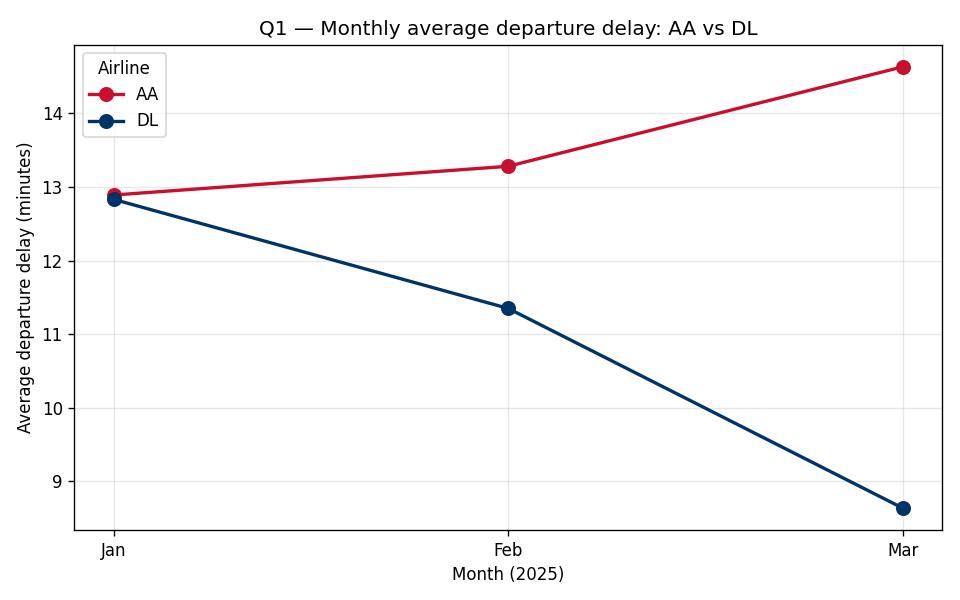
\includegraphics[width=0.49\linewidth]{../plots/q1_avg_dep_delay.png}\hfill
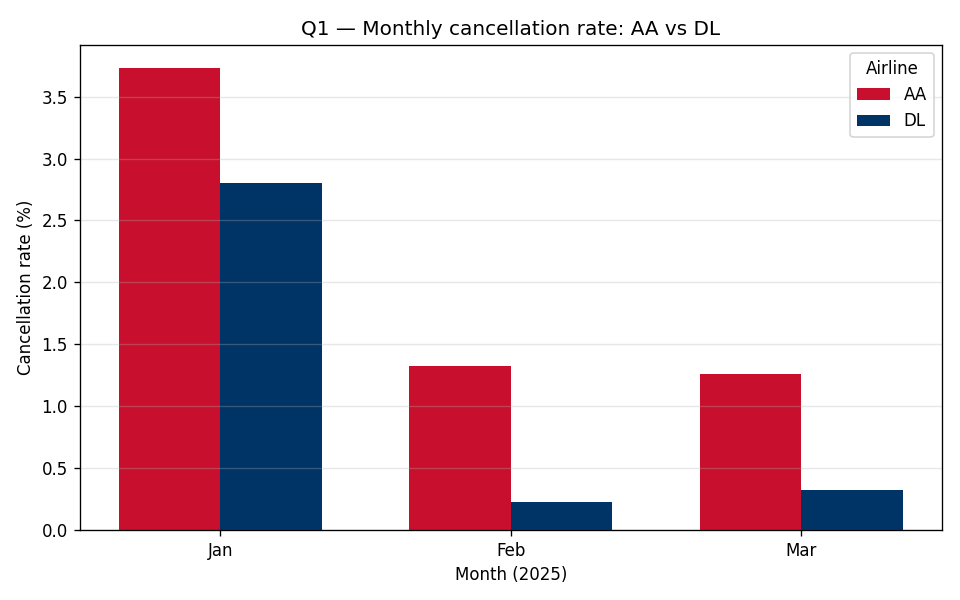
\includegraphics[width=0.49\linewidth]{../plots/q1_cancellation_rate.png}
\caption{Q1: monthly average departure delay (left) and monthly
cancellation rate (right), AA vs DL. Delta consistently posts a
lower cancellation rate than American Airlines, while average
delay is comparable across both carriers and rises in February
and March.}
\label{fig:plots-q1}
\end{figure}

\begin{figure}[h]
\centering
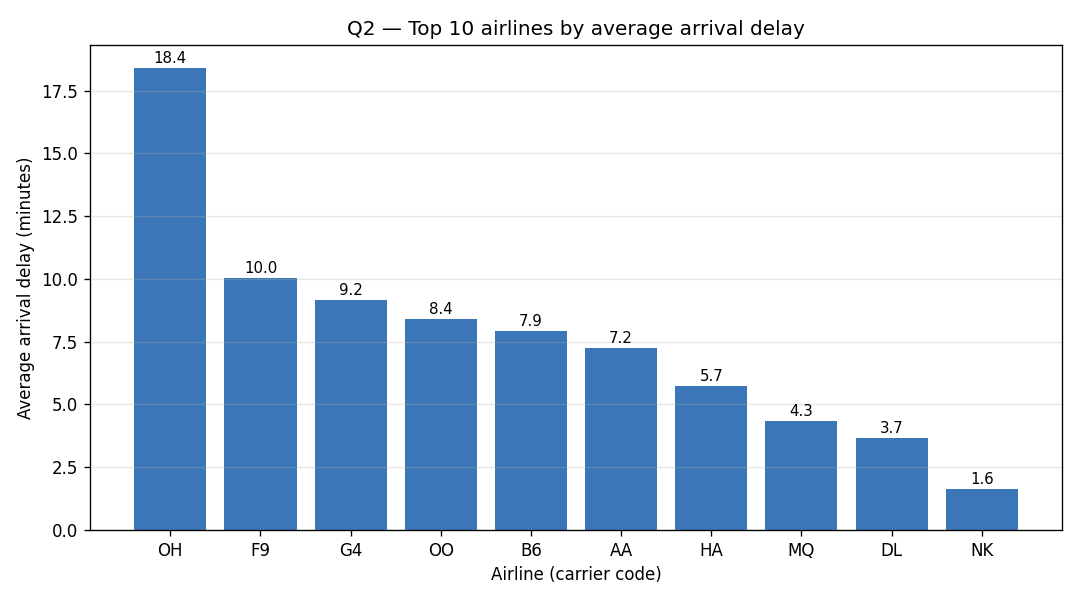
\includegraphics[width=0.49\linewidth]{../plots/q2_top10_ranking.png}\hfill
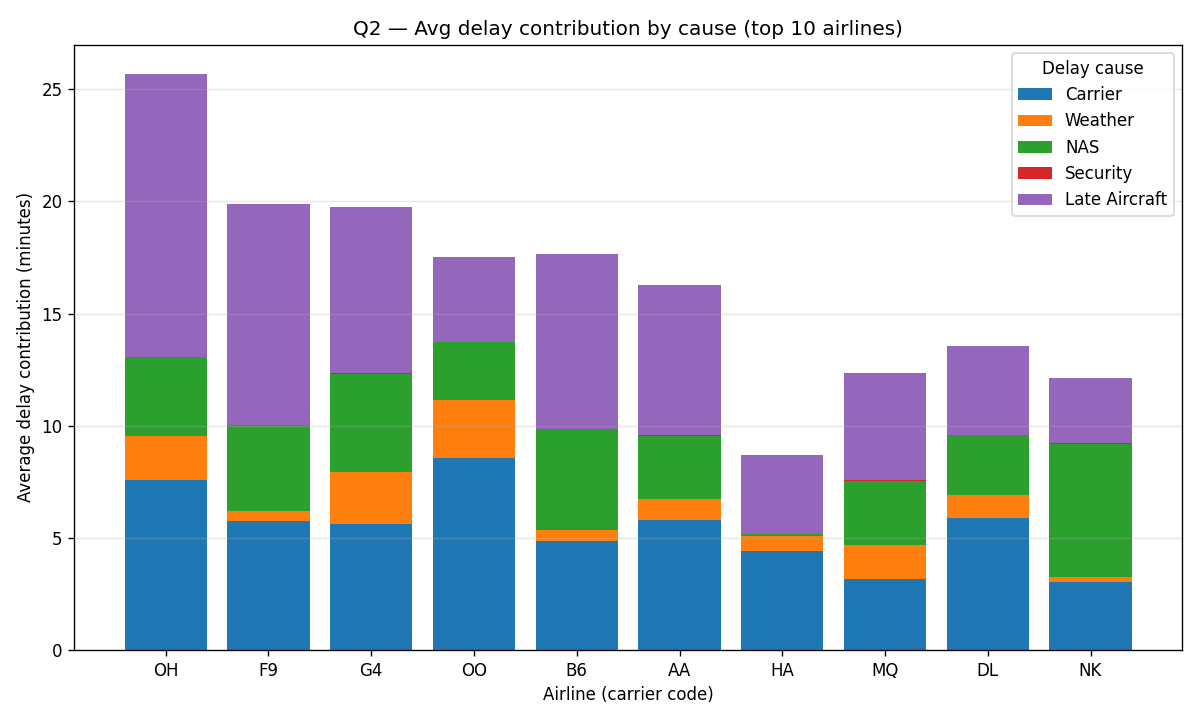
\includegraphics[width=0.49\linewidth]{../plots/q2_delay_causes.png}
\caption{Q2: top~10 carriers by mean arrival delay (left) and the
stacked breakdown of the five delay causes (right). The dominant
contributor for the worst-performing carriers is
\texttt{LATE\_AIRCRAFT\_DELAY}, i.e.\ the cascading effect of
aircraft arriving late from a previous leg.}
\label{fig:plots-q2}
\end{figure}

\subsection{Observations}

\paragraph{HDFS overhead is real and stable}
End-to-end time grows by a factor of $3.2\times$ for Q1 and
$4.4\times$ for Q2 when moving from local to HDFS. The overhead
is dominated by the loading stage ($3.8\times$ for Q1 and a
striking $17\times$ for Q2), reflecting the cost of
communicating with the namenode, fetching block locations and
streaming data from the datanode container. Computation time is
essentially unchanged, as expected: the actual data volume is
small compared to what a single modern CPU can crunch in a few
hundred milliseconds.

\paragraph{Output is the second-largest cost in HDFS}
For Q2 in particular the output stage averages $5.94$\,s. This
is the coalesce-induced final shuffle to a single partition,
combined with the HDFS write path (block write, namenode
metadata update, replication acknowledgment), amplified by
container network latency.

\paragraph{Warmup is non-optional}
A pilot run without warmup measured a Q1 end-to-end of
$34.9$\,s in the HDFS cluster, against a steady-state of
$19.1$\,s. The $\sim$16-second gap is consistent with JVM JIT
compilation kicking in plus HDFS metadata caches warming up,
and it justifies discarding the first iteration when benchmarking.

% -------------------------------------------------------------
\section{Discussion and Lessons Learned}\label{sec:discussion}

\paragraph{Explicit schema pays off}
Letting \texttt{inferSchema=true} adds an entire extra pass over
the CSV just to deduce column types. Declaring the schema
explicitly with \texttt{StructType} approximately halves the
loading time and, as a bonus, prevents subtle silent type
mismatches on columns like \texttt{DEP\_DELAY} which contain
occasional empty values.

\paragraph{\texttt{cache()} only when the DataFrame is reused}
Q1 caches the filtered DataFrame because it feeds two independent
aggregations. Q2 does not, because it consumes the input only
once; adding a \texttt{cache()} call there would only waste
memory and trigger an extra materialization pass without any
downstream consumer.

\paragraph{Shuffle partitions tuned to the workload}
Spark's default of 200 shuffle partitions is overkill for a
working dataset of $1.55$~M records on a single machine. The
configuration is reduced to~8, which lines up with the host CPU
count and removes the scheduling overhead introduced by lots of
mostly-empty partitions.

\paragraph{Coalesce is a UX/cost trade-off}
\texttt{coalesce(1)} guarantees a single CSV file per query (the
project deliverable wants exactly one per query) at the cost of
a trailing shuffle that shows up in the output timer. Dropping
\texttt{coalesce(1)} would shave roughly $1$--$3$\,s but would
also produce eight \texttt{part-*} files that the user would
then have to concatenate by hand.

% -------------------------------------------------------------
\section{Conclusions}\label{sec:conclusion}

This project demonstrates a complete, reproducible Big Data
pipeline that combines HDFS storage and Spark processing, both
deployed via Docker Compose so that the cluster can be brought
up from scratch in under a minute. The two required queries are
implemented with the DataFrame API, paying explicit attention to
lazy evaluation, caching and shuffle behaviour. The experimental
evaluation quantifies what it costs to move from a local PySpark
setup to a containerized HDFS+Spark cluster, and identifies
loading (network and metadata) and output (coalesce + HDFS
replication) as the dominant overhead sources. The full source
code, the result CSVs, the benchmark logs and this report are
organized in a single repository as required by the project
specification.

% -------------------------------------------------------------
\begin{thebibliography}{9}

\bibitem{bts}
US Bureau of Transportation Statistics, ``On-Time Performance
Data,'' \url{https://www.transtats.bts.gov/}, accessed May 2026.

\bibitem{spark}
M. Zaharia \emph{et al.}, ``Apache Spark: A unified engine for
big data processing,'' \emph{Communications of the ACM},
vol.~59, no.~11, pp.~56--65, 2016.

\bibitem{hdfs}
K. Shvachko, H. Kuang, S. Radia, and R. Chansler, ``The Hadoop
Distributed File System,'' \emph{IEEE 26th Symposium on Mass
Storage Systems and Technologies (MSST)}, pp.~1--10, 2010.

\bibitem{docker}
D. Merkel, ``Docker: lightweight Linux containers for consistent
development and deployment,'' \emph{Linux Journal}, vol.~2014,
no.~239, 2014.

\bibitem{bde2020}
Big Data Europe, ``Hadoop and Spark Docker images,''
\url{https://github.com/big-data-europe}, accessed May 2026.

\end{thebibliography}

\end{document}
